\documentclass[10pt, letterpaper]{article}

% Pacotes:
\usepackage[
    ignoreheadfoot,
    top=2 cm,
    bottom=2 cm,
    left=2 cm,
    right=2 cm,
    footskip=1.0 cm,
]{geometry}
\usepackage{titlesec}
\usepackage{tabularx}
\usepackage{array}
\usepackage[dvipsnames]{xcolor}
\definecolor{primaryColor}{RGB}{0, 0, 0}
\usepackage{enumitem}
\usepackage{fontawesome5}
\usepackage{amsmath}
\usepackage{graphicx} % Adicionado para incluir imagens
\usepackage[
    pdftitle={Currículo de João Pinto},
    pdfauthor={João Pinto},
    pdfcreator={LaTeX with RenderCV},
    colorlinks=true,
    urlcolor=primaryColor
]{hyperref}
\usepackage[pscoord]{eso-pic}
\usepackage{calc}
\usepackage{bookmark}
\usepackage{lastpage}
\usepackage{changepage}
\usepackage{paracol}
\usepackage{ifthen}
\usepackage{needspace}
\usepackage{iftex}
\ifPDFTeX
    \input{glyphtounicode}
    \pdfgentounicode=1
    \usepackage[T1]{fontenc}
    \usepackage[utf8]{inputenc}
    \usepackage{lmodern}
\fi
\usepackage{charter}

\raggedright
\AtBeginEnvironment{adjustwidth}{\partopsep0pt}
\pagestyle{empty}
\setcounter{secnumdepth}{0}
\setlength{\parindent}{0pt}
\setlength{\topskip}{0pt}
\setlength{\columnsep}{0.15cm}
\pagenumbering{gobble}

\titleformat{\section}{\needspace{4\baselineskip}\bfseries\large}{}{0pt}{}[\vspace{1pt}\titlerule]

\titlespacing{\section}{
    -1pt
}{0.3 cm}{0.2 cm}

\renewcommand\labelitemi{$\vcenter{\hbox{\small$\bullet$}}$}
\newenvironment{highlights}{
    \begin{itemize}[
        topsep=0.10 cm,
        parsep=0.10 cm,
        partopsep=0pt,
        itemsep=0pt,
        leftmargin=1cm % Indentação adicionada aqui
    ]
}{
    \end{itemize}
}
\newenvironment{subhighlights}{
    \begin{itemize}[
        topsep=0.10 cm,
        parsep=0.10 cm,
        partopsep=0pt,
        itemsep=0pt,
        leftmargin=1.5cm, % Indentação mais profunda
        label=$\vcenter{\hbox{\scriptsize$\circ$}}$ % Estilo diferente para o marcador
    ]
}{
    \end{itemize}
}

\newenvironment{header}{
    \setlength{\topsep}{0pt}\par\kern\topsep\centering\linespread{1}
}{
    \par\kern\topsep
}

\begin{document}

% Cabeçalho
\begin{header}
    % Criar um container horizontal para a foto e o nome
    \begin{minipage}[c]{0.2\textwidth} % Foto à esquerda
        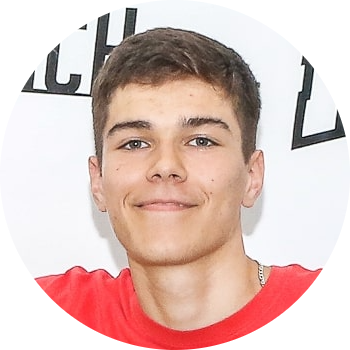
\includegraphics[width=\textwidth]{photo.jpg} % Substitua 'photo.jpg' pela sua foto
    \end{minipage}
    \hfill
\begin{minipage}[c]{0.75\textwidth} % Nome à direita, centralizado verticalmente
    % Nome alinhado ao meio da foto
    {\fontsize{25 pt}{25 pt}\selectfont \textbf{João Pinto}} \\[0.1cm] % Ajuste o espaçamento conforme necessário
    {\fontsize{12 pt}{12 pt}\selectfont Desenvolvedor de Software | \href{https://joaopinto15.github.io}{Website: joaopinto15.github.io}}
\end{minipage}

    
    % Adicionar detalhes de contato abaixo da imagem e do nome
    \vspace{0.8cm} % Espaço entre o nome e os detalhes de contato
    \centering
    \normalsize
    Cidadão PT | 
    \href{mailto:pintojad03@gmail.com}{pintojad03@gmail.com} | 
    \href{tel:+351-915-069-719}{(+351) 915-069-719} | 
    \href{https://linkedin.com/in/joaopinto15}{LinkedIn: joaopinto15} | 
    \href{https://github.com/joaopinto15}{GitHub: joaopinto15}
\end{header}



% Seção de Educação
\section{Formação}
\textbf{\href{https://www.isep.ipp.pt}{Instituto Superior de Engenharia do Porto}} \hfill \textbf{Porto, Portugal} \\
Licenciatura em Engenharia Informática \hfill \textit{Conclusão Prevista: Maio de 2025} \\
\begin{subhighlights}
    \item \textbf{Concentrações:} Projetos de Software e Metodologias Ágeis
    \item \textbf{Nota:} 16.00/20.00
    \item \textbf{Principais Disciplinas:} Estruturas de Dados e Algoritmos, Padrões de Design, Bases de Dados, 
    Redes de Computadores, Sistemas Operativos, Machine Learning, Inteligência Artificial, Programação Orientada a Objetos, SCRUM
\end{subhighlights}

% Seção de Experiências
\section{Experiência}
\begin{highlights}
    \item Atualmente em busca de experiência profissional.
\end{highlights}
% Seção de Projetos
\section{PROJETOS}
\textbf{Hair Drop} \hfill \textbf{Sofia, Bulgária} \\
\textit{Líder de Equipa} \hfill Setembro 2024 \\
\begin{highlights}
    \item Desenvolvimento de aplicação full-stack utilizando Rust (back-end) e React (front-end) com conceitos de código seguro.
    \item Integração de princípios de código seguro: prevenção de injeções SQL, manutenção de vazamentos de memória e proteção de APIs.
\end{highlights}

\textbf{\href{https://purenimble.github.io/projects}{Projetos do ISEP}} \hfill \textbf{Porto, Portugal} \\
\textit{Líder/Membro da Equipa} \hfill Nov 2022 – Jan 2025 \\
\begin{highlights}
    \item Liderança de equipa utilizando metodologias ágeis, gerindo sprints e tarefas da equipa.
    \item Desenvolvimento de aplicação full-stack utilizando Java e C.
\end{highlights}

% Seção de Atividades e Liderança
\section{ATIVIDADES e Liderança}
\textbf{Universidade Técnica de Sofia} \hfill \textbf{Sofia, Bulgária} \\
\textit{Estudante Erasmus+} \hfill Setembro 2024 – Jan 2025 \\
\begin{highlights}
    \item 1 semestre em um programa universitário ministrado em inglês, ganhando exposição académica internacional valiosa.
\end{highlights}

\textbf{Desporto Federado – Basquetebol} \hfill \textbf{Porto, Portugal} \\
\textit{Jogador de Basquetebol} \hfill 2006 – 2022 \\
\begin{highlights}
    \item Desenvolvimento de trabalho em equipa, comunicação e disciplina através do basquetebol competitivo.
    \item Aprendizado de pontualidade, respeito às regras e colaboração em equipa.
\end{highlights}

% Seção de Competências
\section{Competências}
\textbf{Programação:} Java, C, Python, JavaScript, SQL, Node.js, React.js, MATLAB, Rust \\
\textbf{Ferramentas:} Git, Agile, SCRUM, Docker, SSH

\end{document}
